\documentclass[../../lecture_notes.tex]{subfiles}
\begin{document}


Let’s implement our own version of a pipe
\begin{lstlisting}
#define PIPE_SIZE 1<<12
struct pipe {
	char buf[PIPE_SIZE];
	unsigned r, w;
	lock_t *alock;
}
void lock(lock_t* alock);
void unlock(lock_t* alock);
// we ignore the implementation of lock and unlock for now
char readc(struct pipe *p) {
	lock(&l);
	// we cannot hold the lock while the pipe is full; we wait
	while (p->r == p->w) {
		unlock(&l);
		lock(&l);
	}
	char c = p->buf[p->r++ % PIPE_SIZE];
	unlock(&l);
	return c
}
// we do a writec the same way
\end{lstlisting}


This is a fine grain lock; we could use a global lock, but that would be course grain and slow

How do we implement a lock?

We can use the following instruction
\begin{lstlisting}
int xchgl(int* p, int val) {
	int old = *p;
	*p = val;
	return old;
}
\end{lstlisting}

and thus write the following cosine function:
\begin{lstlisting}
void cosine(struct s *p) {
	do {
		double d1 = p->d;
		double d2 = cos(d1);
	} while(xchgl(&p->d, d1, d2) != old);
}
\end{lstlisting}
but the value can change before we run xchgl and cause us to loop infinitely!

We need to use cas!
\begin{lstlisting}
bool cas(int *p, double old, double new) {
	if (*p==old) {*p=new; return 1;}
	else return 0;
}
\end{lstlisting}


We can instead use the command to build a portable 
\begin{lstlisting}
void cosine(struct s *p) {
	do {
		double d1 = p->d;
		double d2 = cos(d1);
	} while(!cas(&p->d, d1, d2);
}
\end{lstlisting}

We can utilize the above commands to abstract a lock API of the following sort:
\begin{lstlisting}
struct s {
	double d;
	lock_t l;
}
void cosine(struct s *p) {
	lock(&s->l);
	p->d = cos(p->d);
	unlock(&p->l);
}
\end{lstlisting}

Maximum performance is found by minimizing the critical section, but we have reached the atomicity of the next layer down, so this is as well as we can do!

This style of lock is still pretty slow; a mutex is more efficient than a spin lock because we sleep while waiting

Let’s try to make one!
\begin{lstlisting}
//Mutex
typedef struct s{
	bool acquired;
	thread_descriptor_t *blocked;
	lock_t lock;
} bmutex_t;
// blocked forms linked list of waiting threads

void acquire(bmutex_t *b) {
	again:
	lock(&b->lock);
	if(!b->acquired) {
		b->acquired = true;
		unlock(&b->lock);
	}
	else {
		self->blocked->blocked = true;
		add_self_to_blocked_queue();
		unlock(&b->lock);
		yield();
		goto again;
	}
}
void release(bmutex *b) {
	b->locked = 0;
	unlock(&b->lock);
}
\end{lstlisting}

We can generalize a mutex to for a number of concurrent threads with a semaphore.

\subsubsection*{Semaphore}

The basics:
\begin{itemize}
\item locked when ctr <= 0
\item ctr = numbers of resources left
\item N threads waiting if ctr = N
\item to lock, increase ctr and place self on queue
\end{itemize}


Eggert is not a huge fan of semaphores, so they were not discussed much. They are effectively a primitive for locks and condition variables. We can, however, use these to prevent thrashing!

We can also use this to solve an earlier problem; if the pipe is empty, neither reading nor writing can be done, since it appears full. This is called the \term{producer/consumer problem}.

SO we abstract from a semaphore to solve it with a condition variable


\subsubsection*{Condition Variable}

A condition variable contains 2 parts:
\begin{enumerate}
\item bool isempty
\item blocking mutex (binary semaphore)
\end{enumerate}


The API is as follows:
\begin{lstlisting}
int pthread_cond_wait(condvar_t *c, bmutex_t *b);
// wait until the condition becomes true
int pthread_cond_signal(condvar_t *c);
// notify the first waiting thread that c is true
int pthread_cond_broadcast(condvar_t *c);
// notify all waiting threads that c is true
// Used for when there are too many variations for separate conditions
\end{lstlisting}

A wake does not guarantee a condition is met; the thread must check again.

We implement one like so
\begin{lstlisting}
struct pipe {
	char buf[BUFSIZ];
	bmutex_t b;
	int r, w;
	condvar_t nonempty;
}
int pipe_read(struct pipe *p) {
	again:
	acquire(&p->b);
	if (p->w == p->r) {
		pthread_cond_signal(&p->nonempty, &p->b);
		goto again;
	}
	char c = p->buf[p->r++%BUF_SIZE];
	release(&p->b);
	notify(&p->nonempty);
	return c;
}
\end{lstlisting}


We can use these ideas to create a few thread-safe data structures:
\begin{enumerate}[nosep]
\item Concurrent Counters:
	\begin{itemize}
		\item Place a lock around access and incrementation
		\item Not perfectly scalable, since multiprocessing greatly increases time cost
	\end{itemize}
\item Scalable Counter:
	\begin{itemize}
		\item Each thread gets its own counter.
		\begin{itemize}
			\item Threads share one global counter, local counters are flushed after set time
			\item Value is $\pm$ n\_threads*flushTime 
			\item Time to flush locks: high = inaccurate, low = not scalable
		\end{itemize}
	\end{itemize}
\item Concurrent Linked Lists: 
	\begin{itemize}
	\item Locking Options:
	\begin{enumerate}
		\item Hand-over-hand/lock coupling
			\begin{itemize}
				\item Each node has its own lock
				\item This is slow, so we usually do not use it
			\end{itemize}
		\item List Locking
			\begin{itemize}
				\item One lock for head and one for tail
				\item Wait if queue is full or empty
			\end{itemize}
	\end{enumerate}
	\end{itemize}
\item Concurrent Hash Table:
	\begin{itemize}
		\item One lock per bucket
		\item Still constant time!
	\end{itemize}
\end{enumerate}

NOTE: With these, we still want to avoid premature optimization

There is still an optimization we can perform for small critical sections for a speedup; we  cheat our way to improving locks with machine code
\begin{lstlisting}[language=sh]
lock:
	movl $1, %eax

unlock:
	xrelease movl $0, mutex

try:
	xacquire lock xchgl %eax, mutex
	cmp $0, %eax
	jne try
	ret
# store edits into a cache & write into memory only on success
\end{lstlisting}
A few observations:
\begin{itemize}
	\item This relies on caching for speed, so critical sections must be sufficiently small
	\item Note that if we did not use test and sleep, we could get a race condition
	\item This makes a single-threaded program slower due to overhead
\end{itemize}

BUT WAIT, we can still get bugs based on usage
\begin{lstlisting}
bool copyc(struct pipe *p, struct pipe *q){
	bool ok = 0;
	acquire(&p->b);
	acquire(&q->b);
	if(p->w - p->r == 0 && q->w - q->r != 1024){
		q->buff[q->w++%1024] = p->buf[p->r++%1024];
		ok = 1;
	}
	release(&p->b);
	release(&q->b);
	return ok;
}
// multiple threads could end up waiting on each other, and the program halts
\end{lstlisting}

This situation is called a

\subsection{Deadlock}

There are four condition for deadlock:
\begin{enumerate}
	\item \term{circular wait} $\coloneqq$ there is a cycle of dependencies
	\item \term{mutual exclusion} $\coloneqq$ threads claim exclusive control of required resources
	\item \term{no preemption of locks} $\coloneqq$ resources cannot be forcefully taken from threads
	\item \term{hold \& wait} $\coloneqq$ threads hold resources while waiting for more
\end{enumerate}

We have a few ways to avoid deadlocks (besides just using lock-free and wait-free data structures)
\begin{enumerate}
\item Dynamic Deadlock Detection
\begin{itemize}
	\item The OS checks for possible deadlock in any thread on request \& EDEADLOCK on fail
	\item This pushes deadlock handling onto the app; if there is a deadlock, the OS just gives up
\end{itemize}
\item Lock Ordering
\begin{itemize}
	\item assign a priority to each lock (often by address)
	\item always lock objects in order of priority
	\item wait on first lock failure but release all and try again if a later one fails
\end{itemize}
\item Intervention
\begin{itemize}
	\item kill deadlocked threads
	\item is used much too often
\end{itemize}
\end{enumerate}


There are some types of deadlock that don’t fit neatly into any solution
\begin{enumerate}
\item Parent/Child Communication \\
	If the two threads communicate via two pipes and both write a lot and don’t read, both may wait on a full pipe!
\item Priority Inversion \\
	\begin{minipage}{0.7\linewidth}
	\begin{itemize}
	\item High priority thread needs a lock
	\item Low priority thread has that lock
	\item Low priority thread is waiting on mid priority
	\end{itemize}
	Then the high priority is waiting on the mid and low!
	\end{minipage}%
	\begin{minipage}{0.3\linewidth}
	\centering
	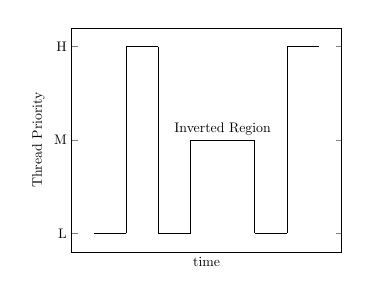
\begin{tikzpicture}[scale=0.5]
	\begin{axis}[ 
		xmajorticks=false, ytick={1,2,3}, yticklabels={L, M, H}, xlabel={time}, ylabel={Thread Priority}
	]
		\addplot[domain=0:1] {1};
		\addplot[domain=1:3] (1, x);
		\addplot[domain=1:2] {3};
		\addplot[domain=1:3] (2, 4-x);
		\addplot[domain=2:3] {1};
		\addplot[domain=1:2] (3, x);
		\addplot[domain=3:5] {2} node[pos=0.5, above] {Inverted Region};
		\addplot[domain=1:2] (5, 3-x);
		\addplot[domain=5:6] {1};
		\addplot[domain=1:3] (6, x);
		\addplot[domain=6:7] {3};
	\end{axis}
	\end{tikzpicture}
	\end{minipage}
	
	SOLUTION: \\
	threads gain the priority of the highest priority dependent thread
\end{enumerate}


We can also be stopped by \term{live-lock} $\coloneqq$ when the thread is trying to run but failing.

\begin{minipage}{0.7\linewidth}
For example, an inundated router may spend most of its time accepting requests, since they come via interrupt, and never actually fulfill any requests. We have two possible solutions:
\begin{enumerate}[nosep]
\item if router fills, toss requests until the router hits a low threshold
\item if requests are above a threshold, block interrupts 
\end{enumerate}
\end{minipage}%
\begin{minipage}{0.3\linewidth}
\centering
\begin{tikzpicture}[scale=0.5]
\begin{axis} [
	axis lines*=left, ticks=none, xlabel={Work Done}, ylabel={Load}, axis equal
]
\addplot[domain=0:5, dashed] {1} node[pos=0.5, above] {CPU limit};
\addplot[domain=0:5, smooth] {1-1/x};
\addplot[domain=1:5, smooth] {2*(cos(45*(x-1)) - 1)};
\addplot[domain=0:1, variable=\t, Latex-Latex] ({3}, {2/3 - 8/3*t)}) 
	node[pos=0.5, right, align=center, scale=0.75] {Interrupt\\handler\\work};
\end{axis}
\end{tikzpicture}
\end{minipage}

We discuss two of the most common non-deadlock bugs:
\begin{enumerate}
\item \term{atomicity violation} $\coloneqq$ code has an implied atomicity which is violated. This involves an \term{atomicity assumption} of a non-atomic action. This can be solved by locks!
\begin{lstlisting}
// Thread 1::
if (thd->proc_info) {
	fputs(thd->proc_info, ...);
}

// Thread 2::
thd->proc_info = NULL;
\end{lstlisting}

\item \term{order violation} $\coloneqq$ the desired order of two memory accesses is flipped. This usually involves trying to act on a variable that is inialized in another thread. This can be solved by semaphores.
\begin{lstlisting}
// Thread 1::
void init() {
	nThread = PR_CreateThread(nMain, ...);
}

// Thread 2::
void nMain(...) {
	nState = nThread->State;
}
\end{lstlisting}
\end{enumerate}


\end{document}